\item A bola de bilhar $A$ move-se com uma velocidade de \SI{10}{\meter/\second} imediatamente antes de atingir a bola $B$, que está em repouso. Se as massas de $A$ e $B$ são \SI{200}{\gram} cada e o coeficiente de restituição entre eles é $e=0.8$, determine a velocidade de ambas as bolas logo após o impacto.

\begin{flushright}
	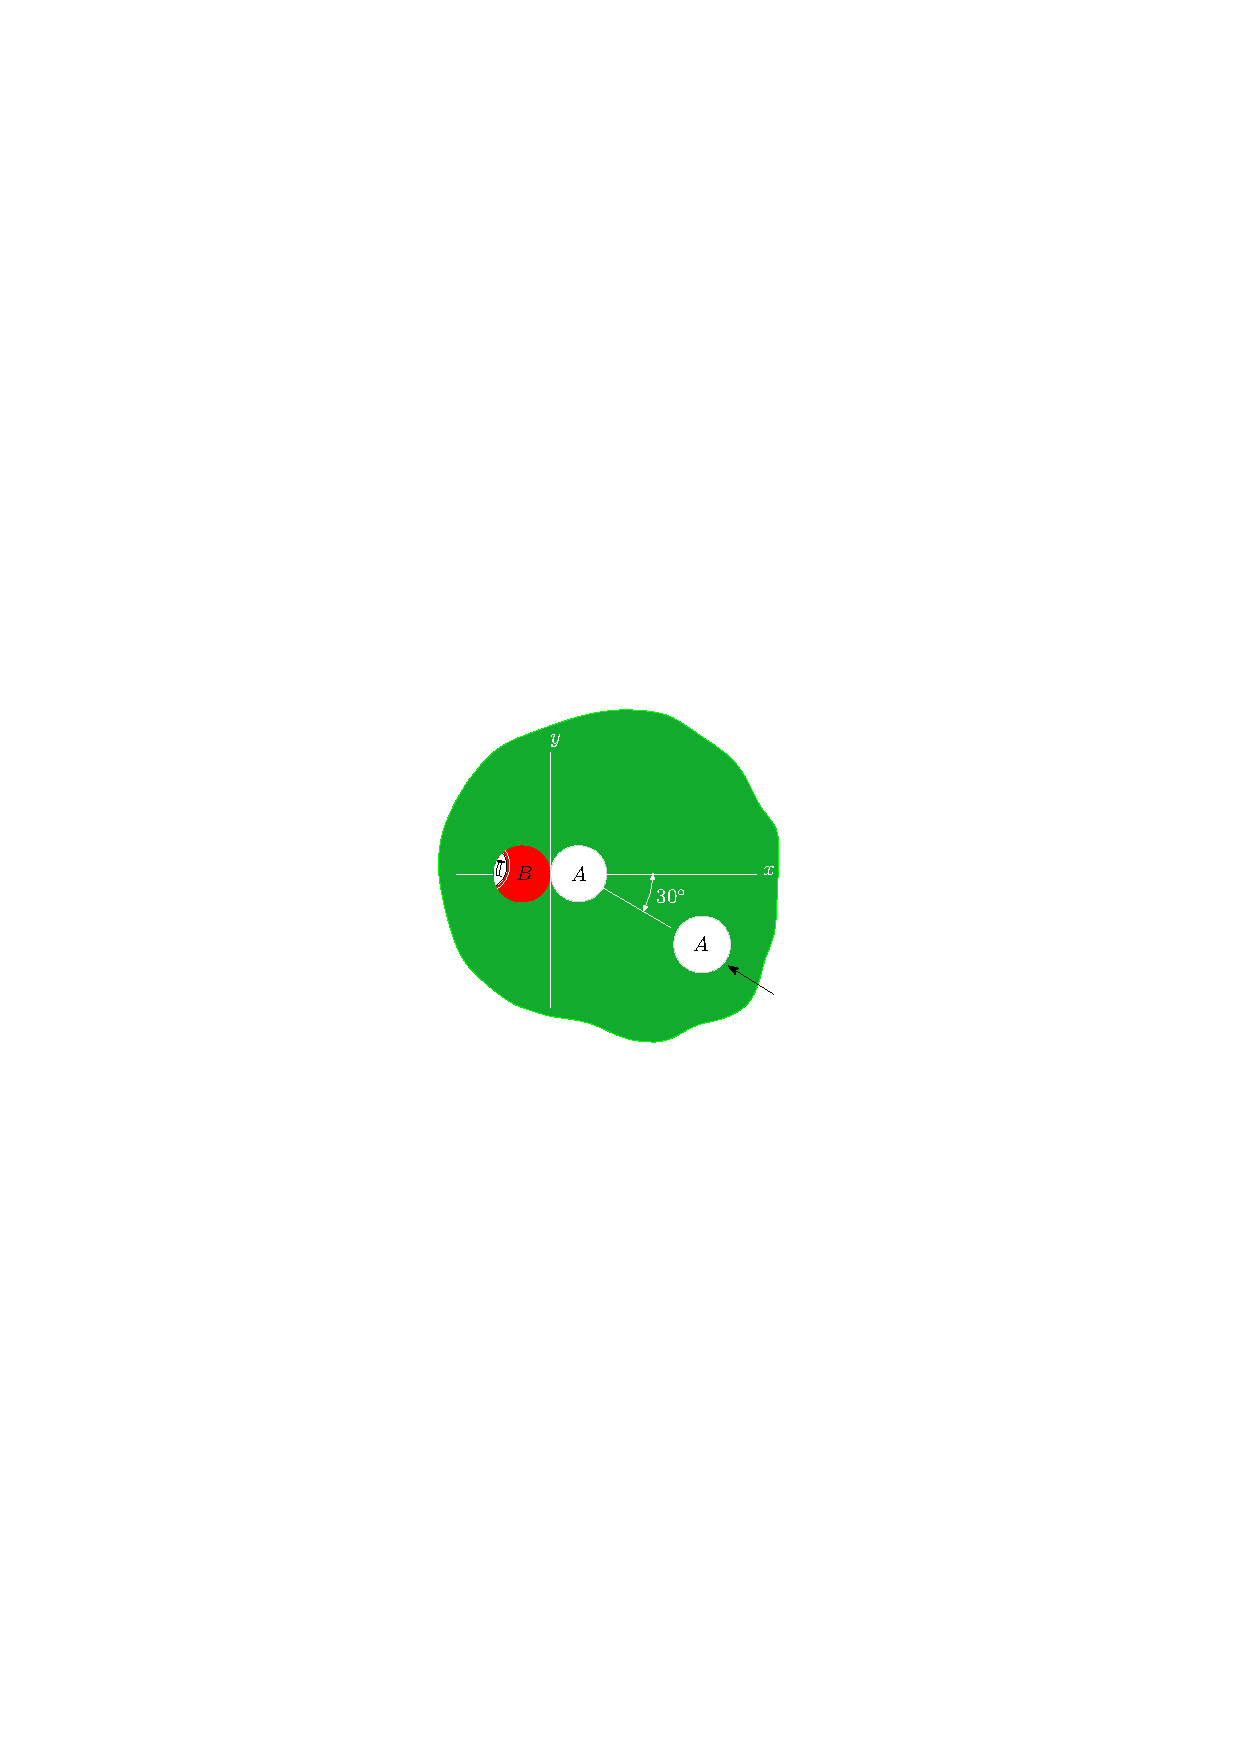
\includegraphics[scale=1.4]{images/draw_11}
\end{flushright}